\documentclass[]{article}
\usepackage{amsmath}
\usepackage{amssymb}
\usepackage{amsthm}
\usepackage{indentfirst}
\usepackage{tikz}
\usetikzlibrary{arrows,automata}
\begin{document}

\title{COMS W3261 \\ Computer Science Theory \\ Chapter 2 Notes}
\author{Alexander Roth}
\date{2014-09-06}
\maketitle

\section*{Definitions}
  \begin{description}
    \item[Deterministic] The automaton cannot be in more than one state at any
    time.
    \item[Nondeterministic] The automaton may be in several states at once.
  \end{description}

\section*{An Informal Picture of Finite Automata}
  We will be using the example of a real-world problem whose solution uses
  finite automata in an important role. We investigate protocols that support
  ``electronic money'' -- files that a customer can use to pay for goods on
  the internet, and that the seller can receive insurance that the ``money''
  is real.

  \subsection*{The Ground Rules}
    There are three participants: the customer, the store, and the bank. We
    assume for simplicity that there is only one ``money'' file in existence.
    Interactions among the three participants is thus limited to five
    elements:
    \begin{enumerate}
      \item The customer may decide to \emph{pay}. That is, the customer sends
      the money to the store.
      \item The customer may decide to \emph{cancel}. The money is sent to the
      bank with a message that the value of the money is to be added to the
      customer's bank account.
      \item The store may \emph{ship} goods to the customer.
      \item The store may \emph{redeem} the money. That is, the money is sent
      to the bank with a request that its value be given to the store.
      \item The bank may \emph{transfer} the money by creating a new, suitably
      encrypted money file and sending it to the store.
    \end{enumerate}

  \subsection*{The Protocol}
    The customer cannot be relied upon to act responsibly. In particular, the
    customer may try to copy the money file, use it to pay several times, or
    both pay and cancel the money, thus getting the goods ``for free''. The
    bank must behave responsibly, or it cannot be a bank. The store should be
    careful as well. In particular, it should not ship goods until it is sure
    it has been given valid money for the goods. \\
    \indent These types of protocols can be represented by finite automata.
    Each state represents a situation that one of the participants could be
    in. Transitions between states occur when one of the five events described
    above occur. \\

    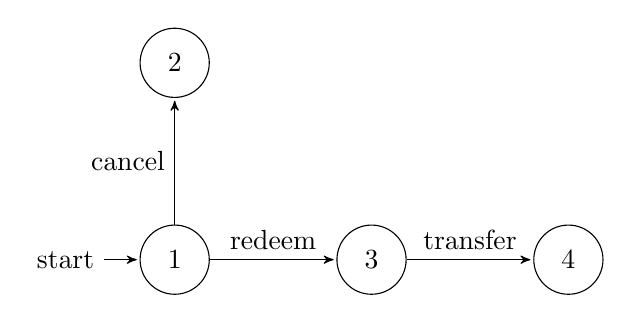
\begin{tikzpicture}[>=stealth',shorten >=1pt,auto,node distance=2.5cm]
      \node[initial,state] (1)              {$1$};
      \node[state]         (2) [above of=1] {$2$};
      \node[state]         (3) [right of=1] {$3$};
      \node[state]         (4) [right of=3] {$4$};

      \path[->] (1) edge node {cancel}   (2);
      \path[->] (1) edge node {redeem}   (3);
      \path[->] (3) edge node {transfer} (4);
    \end{tikzpicture}

    This is the automaton for the bank. The start state is state 1; it
    represents the situation where the bank has issued the money file in
    question but has not been requested either to redeem or cancel it. If a
    \emph{cancel} request is sent to the bank by the customer, then the bank
    restores the money to the customer's account and enters state 2. The bank,
    being responsible, will not leave state 2 once it is entered, since the
    bank must not allow the same money to be cancelled again or spent by the
    customer. Similar concepts should be applied to the other states. \\
    \indent Now, let us consider the automaton of the actions for the store.\\

    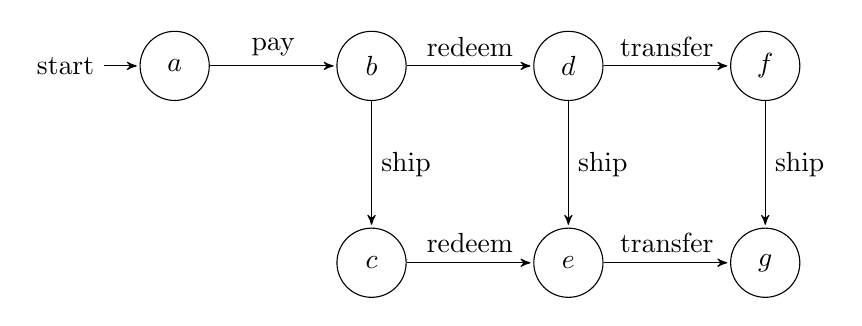
\begin{tikzpicture}[>=stealth',shorten >=1pt,auto,node distance=2.5cm]
      \node[initial,state] (a)              {$a$};
      \node[state]         (b) [right of=a] {$b$};
      \node[state]         (c) [below of=b] {$c$};
      \node[state]         (d) [right of=b] {$d$};
      \node[state]         (e) [below of=d] {$e$};
      \node[state]         (f) [right of=d] {$f$};
      \node[state]         (g) [below of=f] {$g$};

      \path[->] (a) edge node {pay}      (b);
      \path[->] (b) edge node {ship}     (c);
      \path[->] (b) edge node {redeem}   (d);
      \path[->] (c) edge node {redeem}   (e);
      \path[->] (d) edge node {ship}     (e);
      \path[->] (d) edge node {transfer} (f);
      \path[->] (e) edge node {transfer} (g);
      \path[->] (f) edge node {ship}     (g);
    \end{tikzpicture}

    There are some defects in the store's design. Imagine that the shipping
    and financial operations are done by separate processes, so there is the
    opportunity for the \emph{ship} action to be done either before, after, or
    during the redemption of the electronic money. Thus, the store can get
    into situations where it has already shipped the goods only to find out
    that the money was bogus. \\
    \indent Finally, there is the automaton for the customer.

    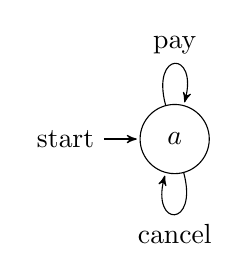
\begin{tikzpicture}[>=stealth',shorten >=1pt,auto,node distance=2.5cm]
      \node[initial, state] (a) {$a$};

      \path[->] (a) edge [loop above] node {pay}    (a);
      \path[->] (a) edge [loop below] node {cancel} (a);
    \end{tikzpicture}

    This automaton only has one state, reflecting the fact that the customer
    ``can do anything.'' The customer can perform the \emph{pay} and
    \emph{cancel} actions any number of times, in any order, and stays in the
    lone state after each action.

  \subsection*{Enabling the Automata to Ignore Actions}
    While the three automata reflect the behaviors of the three participants
    independently, there are certain transitions that are missing. For
    example, the store is not affected by a \emph{cancel} message. According
    to the formal definition of a finite automaton, whenever an input $X$ is
    received by an automaton, the automaton must follow an arc labeled $X$
    from the state it is in to some new state. \\
    \indent Thus, in the current scenario, if the store were to receive a
    \emph{cancel} action from the customer, the store automaton would ``die'';
    that is, the automaton would be in no state at all, and further actions by
    that automaton would be impossible. This gives rise to the actions that
    must be ignored by an automaton:
    \begin{enumerate}
      \item \emph{Actions that are irreleveant to the participant involved.}
      \item \emph{Actions that must not be allowed to kill the automaton.}
    \end{enumerate}

\section*{Deterministic Finite Automata}
  The term ``deterministic'' refers to the fact that on each input there is
  one and only one state to which the automaton can transition from its
  current state. In contrast, ``nondeterministic'' can be in several states at
  once.

  \subsection*{Definition of a Deterministic Finite Automaton}
    A \emph{deterministic finite automaton} consists of:
    \begin{enumerate}
      \item A finite set of \emph{states}, often denoted by $Q$.
      \item A finite set of \emph{input symbols}, often denoted by $\Sigma$.
      \item A \emph{transition function} that takes as arguments a state and
      an input symbol and returns a state. The transition function will be
      commonly noted as $\delta$. If $q$ is a state, and $a$ is an input
      symbol, then $\delta(q, \, a)$ is the state $p$ such that there is an
      arc labeled $a$ from $q$ to $p^2$.
      \item A \emph{start state}, one of the states in $Q$.
      \item A set of \emph{final} or \emph{accepting} states $F$. The set $F$
      is a subset of $Q$.
    \end{enumerate}
    In proofs, we often talk about a DFA in ``five-tuple'' notation:

      \[ A = (Q, \Sigma, \delta, q_0, F) \]

    where $A$ is the name of the DFA, $Q$ is its set of states, $\Sigma$ its
    input symbols, $\delta$ its transition function, $q_0$ its start state,
    and $F$ its set of accepting states.

  \subsection*{How a DFA Processes Strings}
    The ``language'' of a DFA is the set of all strings that the DFA accepts.
    Suppose $a_{1}a_{2}\cdots a_n$ is a sequence of input symbols. We start
    our DFA in its start state, $q_0$. We consult the transition function
    $\delta$, say $\delta(q_0, a_1) = q_1$ to find the state that the DFA $A$
    enters after processing the first input symbol $a_1$. We continue in this
    manner, finding states $q_2,q_3,\cdots,q_n$ such that $\delta(q_{i-1},
    a_i) = q_i$ for each $i$. If $q_n$ is a member of $F$, then the input
    $a_{1}a_{2}\cdots a_n$ is accepted, and if not then it is ``rejected''.

  \subsection*{Simpler Notations for DFA's}
    There are two preferred notations for describing automata:
    \begin{enumerate}
      \item A \emph{transition diagram}, which is a graph such as the ones
      construct earlier.
      \item A \emph{transition table}, which is a tabular listing of $\delta$
      function, which by implication tells us the set of states and the input
      alphabet.
    \end{enumerate}

    \subsubsection*{Transition Diagrams}
      A \emph{transition diagram} for a DFA $A = (Q, \Sigma, \delta, q_0, F)$
      is a graph defined as follows:
      \begin{enumerate}
        \item[a)] For each state in $Q$ there is a node.
        \item[b)] For each state $q$ in $Q$ and each input symbol $a$ in $
        \Sigma$, let $\delta(q, a) = p.$ Then the transition diagram has an
        arc from node $q$ to node $p$, labeled $a$. If there are several input
        symbols that cause transitions from $q$ to $p$, then the transition
        diagram can have one arc, labeled by the list of these symbols.
        \item[c)] There is an arrow into the start state $q_0$, labeled
        \emph{Start}. This arrow does not originate at any node.
        \item[d)] Nodes corresponding to accepting states (those in $F$) are
        marked by a double circle. States not in $F$ have a single circle.
      \end{enumerate}

    \subsubsection*{Transition Tables}
      A \emph{transition table} is a conventional, tabular representation of a
      function like $\delta$ that takes two arguments and returns a value. The
      rows of the table correspond to the states, and the columns correspond
      to the input. The entry for the row corresponding to state $q$ and the
      column corresponding to input $a$ is the state $\delta(q,a)$. The start
      state is marked with an arrow, and the accepting state is marked with a
      star.

  \subsection*{Extending the Transition Function to Strings}
    We need to make the notion of the language of a DFA precise. Thus, we
    define an \emph{extended transition function} that describes what happens
    when we start in any state and follow any sequence of inputs. If $\delta$
    is our transition function, then the extended transition function
    constructed from $\delta$ will be called $\hat{\delta}$. The extended
    transition function is a function that takes a state $q$ and a string $w$
    and returns a state $p$ -- the state that the automaton reaches when
    starting in state $q$ and processing the sequence of inputs $w$.

  \subsection*{The Language of a DFA}
    Now, we can define the \emph{language} of a DFA $A = (Q, \Sigma, \delta,
    q_0, F)$. This language is denoted $L(A)$, and is defined by

      \[ L(A) = \{w\, | \, \hat{\delta}(q_0, w) \, \text{is in} \, F\} \]

    That is, the language of $A$ is the set of strings $w$ that take the start
    state $q_0$ to one of the accepting states. If $L$ is $L(A)$ for some DFA
    $A$, then we say $L$ is a \emph{regular language}

\section*{Nondeterministic Finite Automata}
  A ``nondeterministic'' finite automaton (\emph{NFA}) has the power to be in
  serval states at once. This ability is often expressed as an ability to
  ``guess'' something about its input. \\
  \indent NFA's accept exactly the regular languages, just as DFA's do.
  However, NFA's are often more succinct and easier to design than DFA's.
  Moreover, while we can always convert an NFA to a DFA, the latter may have
  exponentially more staten than the NFA.

  \subsection*{An Informal View of Nondeterministic Finite Automata}
    An NFA, like a DFA has a finite set of states, input symbols, a start
    state and a set of accepting states. It also has a transition function
    referred to by $\delta$. However, in an NFA, $\delta$ can return a set of
    zero, one, or more states, rather than exactly one.

  \subsection*{Definition of Nondeterministic Finite Automata}
    An NFA is represented essentially like a DFA:

      \[ A = (Q, \Sigma, \delta, q_0m F) \]

    where:
      \begin{enumerate}
        \item $Q$ is a finite set of \emph{states}.
        \item $\Sigma$ is a finite set of \emph{input symbols}.
        \item $q_0$, a member of $Q$, is the \emph{start state}.
        \item $F$, a subset of $Q$, is the set of \emph{final} (or
        \emph{accepting}) states.
        \item $\delta$, the \emph{transition function} is a function that
        takes a state in $Q$ and an input symbol in $\Sigma$ as arguments and
        returns a subset of $Q$.
      \end{enumerate}

  \subsection*{The Extended Transition Function}
    We need to extend the transition function $\delta$ of an NFA to a function
    $\hat{\delta}$ that takes a state $q$ and a string of input symbols $w$,
    and returns the set of states that the NFA is in if it starts in state $q$
    and processes the string $w$.

  \subsection*{The Language of an NFA}
    An NFA accepts a string $w$ if it is possible to make any sequence of
    choices of next state, while reading the characters of $w$, and go from
    the start state to any accepting state. The fact that other choices using
    the input symbols of $w$ lead to a nonaccepting state, or do not lead to
    any state at all (i.e., the sequence of states ``dies''), does not prevent
    $w$ from being accepted by the NFA as a whole. Formally, if $A = (Q,
    \Sigma, \delta, q_0, F)$ is an NFA, then

      \[
        L(A) = \{ \, w \, | \, \hat{\delta}(q_0, w) \, \cap \, F \neq
        \emptyset \}
      \]

    That is, $L(A)$ is the set of string $w$ in $\Sigma^*$ such that $
    \hat{\delta}(q_0, w)$ contains at least one accepting state.

  \subsection*{Equivalence of Deterministic and Nondeterministic Finite
  Automata}
    DFA's and NFA's in practice have about the same number of states, although
    the DFA will will often have more transitions. In the worst case, however,
    the smallest DFA can have $2^n$ states while the smallest NFA for the same
    language has only $n$ states. \\
    \indent The proof that DFA's can do whatever NFA's can do involves an
    important ``construction'' called the \emph{subset construction} because
    it involves constructing all subsets of the set of state of the NFA. \\
    \indent The subset construction starts from an NFA $N = (Q_N, \Sigma,
    \delta_N, q_0, F_N)$. ITs goal is the description of a DFA $D = (Q_D,
    \Sigma, \delta_D, \{q_0\}, F_D)$ such that $L(D) = L(N)$. The other
    components of $D$ are constructed as follows:
      \begin{itemize}
        \item $Q_D$ is teh set of subsets of $Q_N$; i.e., $Q_D$ is the
        \emph{power set} of $Q_N$. Note that if $Q_N$ has $n$ states, then
        $Q_D$ will have $2^n$ states. Often, not all these states are
        accessible from the start state of $Q_D$. Inaccessible states can be
        ``thrown away,'' so effectively, the number of states of $D$ may be
        much smaller than $2^n$.
        \item $F_D$ is the set of subsets $S$ of $Q_N$ such that $S \cap F_N \
        \neq \emptyset$. That is, $F_D$ is all sets of $N$'s states that
        include at least one accepting state of $N$.
        \item For each set $S \subseteq Q_N$ and for each input symbol $a$ in
        $\Sigma$,

          \[
            \delta_D(S, a) \, = \, \bigcup_{p \, \text{in} \, S} \,
            \delta_N(p,a)
          \]

        That is, to compute $\delta_D(S,a)$ we look at all the states $p$ in
        $S$, see what states $N$ goes to from $p$ on input $a$, and take the
        union of all those states.
      \end{itemize}
      \begin{description}
        \item[Theorem:] If $D = (Q_D, \Sigma, \delta_D, \{q_0\}, F_D)$ is the
        DFA constructed from NFA $N = (Q_N, \Sigma, \delta_N, q_0, F_N)$ by
        the subset construction, then $L(D) = L(N)$.
        \item[Theorem:] A language $L$ is accepted by some DFA if and only if
        $L$ is accepted by some NFA.
      \end{description}

  \subsection*{The Pigeonhole Principle}
    Colloquially, if you have more pigeons than pigeonholes, and each pigeon
    files into some pigeonhole, then there must be at least one hole that has
    more than one pigeon. \\
    \indent The pigeonhole principle may appear obvious, but it actually
    depends on the number of pigeonholes being finite. Thus, it works for
    finite-state automata, with the states as pigeonholes, but does not apply
    other kinds of automata that have an infinite number of states.

  \subsection*{Dead States and DFA's Missing Some Transitions}
    We have formally defined a DFA to have a transition from any state, on any
    input symbol, to exactly one state. However, sometimes, it is more
    convenient to design the DFA to ``die'' in situations where we know it is
    impossible for any extension of the input sequence to be accepted.
    Technically, this automaton is not a DFA, because it lacks transitions on
    most symbols from each of its states. \\
    \indent However, such an automaton is an NFA. If we use the subset
    construction to convert it to a DFA, the automaton looks almost the same,
    but it includes a \emph{dead state}, that is, a nonaccepting state that
    goes to itself on every possible input symbol. The dead state corresponds
    to $\emptyset$, the empty set of states of the automaton. \\
    \indent In general, we can add a dead state to any automaton that has
    \emph{no more} than one transition for any state and input symbol. Then,
    add a transition to the dead state from each other state $q$, on all input
    symbols for which $q$ has no other transition. The result will be a DFA in
    the strict sense.

\section*{Finite Automata With Epsilon-Transitions}
  We now allow a transition on $\epsilon$, the empty string. In effect, an NFA
  is allowed to make a transition spontaneously, without receiving an input
  symbol. Like nondeterminism, this new capability does not expand the class
  of languages that can be accepted by finite automata, but it does give us
  some added ``programming convenience''.

  \subsection*{The Formal Notation for an $\epsilon$-NFA}
    We represent an $\epsilon$-NFA exactly as we do an NFA, with one
    exception: the transition function must include information about
    transitions on $\epsilon$. Formally, we represent an $\epsilon$-NFA $A$ by
    $A = (Q, \Sigma, \delta, q_0, F)$, where all components have their same
    interpretation as for an NFA, except that $\delta$ is now a function that
    takes as arguments:
      \begin{enumerate}
        \item A state in $Q$, and
        \item A member of $\Sigma \cup \{\epsilon\}$, that is, either an input
        symbol, or the symbol $\epsilon$.
      \end{enumerate}

  \subsection*{Epsilon-Closures}
    Informally, we $\epsilon$-close a state $q$ by following all transitions
    out of $q$ that are labelled $\epsilon$. However, when we get to other
    states by following $\epsilon$, we follow the $\epsilon$-transitions out
    of those states, and so on, eventually finding every state that can be
    reached from $q$ along any path whose arcs are all labeled $\epsilon$.

  \subsection*{Extended Transitions and Languages for $\epsilon$-NFA's}
    Suppose that $E = (Q, \Sigma, \delta, q_0m F)$ is an $\epsilon$-NFA. We
    first define $\hat{\delta}$, the extended transition function, to reflect
    what happens on a sequence of inputs. The intent is that $\hat{\delta}(q,
    w)$ is the set of states that can be reached along a path whose labels,
    when concatenated, form the string $w$. As always, $\epsilon$'s along this
    path do not contribute to $w$. \\
    \indent The language of an $\epsilon$-NFA $E = (Q, \Sigma, \delta, q_0, F)
    $ is defined as: $L(E) = \{ \, w \, | \, \hat{\delta}(q_0, w) \cap F \neq
    \emptyset$. That is, the language of $E$ is the set of strings $w$ that
    take the start state to at least one accepting state.

  \subsection*{Eliminating $\epsilon$-Transitions}
    Given any $\epsilon$-NFA $E$, we can find a DFA $D$ that accepts the same
    language as $E$. Let $E = (Q_E, \Sigma, \delta_E, q_0, F_E)$. Then, the
    equivalent DFA

      \[ D = (Q_D, \Sigma, \delta_D, q_D, F_D) \]

    is defined as follows:
      \begin{enumerate}
        \item $Q_D$ is the set of subsets of $Q_E$.
        \item $q_D = \, \text{ECLOSE}(S)$; that is, we get the start state of
        $D$ by closing the set consisting of only the start state of E.
        \item $F_D$ is those set of states that contain at least one accepting
        state of $E$. That is, $F_D = \{ \, S \, | \, S \, \text{is in} \, Q_D
        \, \text{and} \, S \cap F_E \neq \emptyset \, \}$.
        \item $\delta_D(S,a)$ is computed, for all $a$ in $\Sigma$ and sets $S
        $ in $Q_D$ by:
          \begin{enumerate}
            \item Let $S = \{p_1, p_2, \ldots, p_k\}$.
            \item Compute $\bigcup^k_{i=1} \delta_E(p_i,a)$; let this set be
            $\{r_1, r_2, \ldots, r_m\}$.
            \item Then $\delta_D(S,a) = \, \text{ECLOSE}(\{r_1,r_2,\ldots,r_m
            \})$.
          \end{enumerate}
      \end{enumerate}
      \begin{description}
        \item[Theorem:] A language $L$ is accepted by some $\epsilon$-NFA if
        and only if $L$ is accepted by some DFA.
      \end{description}

\section*{Summary of Chapter 2}
  \begin{description}
    \item[Deterministic Finite Automata] A DFA has a finite set of states and
    a finite set of input symbols. One state is designated the start state,
    and zero or more states are accepting states. A transition function
    determines how the state changes each time an input symbol is processed.
    \item[Transition Diagrams] It is convenient to represent automata by a
    graph in which the nodes are the states, and arcs are labeled by input
    symbols, indicating the transitions of that automaton. The start state is
    designated by an arrow, and the accepting states by double circles.
    \item[Language of an Automaton] The automaton accepts strings. A string is
    accepted if, starting in the start state, the transitions caused by
    processing the symbols of that string one-at-a-time lead to an accepting
    state. In terms of the transition diagram, a string is accepted if it is
    the label of a path from the start state to some accepting state.
    \item[Nondeterministic Finite Automata] The NFA differs from the DFA in
    that the NFA can have any number of transitions (including zero) to next
    states from a given state on a given input symbol.
    \item[The Subset Construction] By treating sets of states of an NFA as
    states of a DFA, it is possible to convert any NFA to a DFA that accepts
    the same language.
    \item[$\epsilon$-Transitions] We can extend the NFA by allowing
    transitions on an empty input, i.e., no input symbol at all. These
    extended NFA's can be converted to DFA's accepting the same language.
  \end{description}

\end{document}
